% \documentclass[a4paper,journal]{IEEEtran}
\documentclass[conference]{IEEEtran}
%% INFOCOM 2013 addition:
\makeatletter
\def\ps@headings{%
\def\@oddhead{\mbox{}\scriptsize\rightmark \hfil \thepage}%
\def\@evenhead{\scriptsize\thepage \hfil \leftmark\mbox{}}%
\def\@oddfoot{}%
\def\@evenfoot{}}
\makeatother
\pagestyle{headings}
\usepackage{psfrag}

% \usepackage{auto-pst-pdf}

%for using the therefore symbol
\usepackage{amssymb}
%end


\usepackage[utf8]{inputenc}
\usepackage{graphicx}
\usepackage{float}
\usepackage{color, colortbl}
\usepackage{xcolor}
\usepackage{array}
\usepackage{multirow}
\usepackage{footnote}
\usepackage{cite}
%The below is used to add notes to tables without disrupting the IEEEtran format
\usepackage{threeparttable}

% Disable below if wanting to comply exclusively to conference mode of IEEEtran
% \IEEEoverridecommandlockouts

\makesavenoteenv{tabular}

%Ignores \vbox errors below the level of 10000
% \vbadness=10000



\begin{document}
%opening
 \title{Technical report: WMP-Editor}


%A more simple output, useful when involving people from different affiliations
  %\author{
    %  \IEEEauthorblockN{Luis Sanabria-Russo\IEEEauthorrefmark{0}, Jaume Barcelo\IEEEauthorrefmark{0}, Boris Bellalta\IEEEauthorrefmark{0}}\\
      %\IEEEauthorblockA{\IEEEauthorrefmark{0}Universitat Pompeu Fabra, Barcelona, Spain
      %\\\{luis.sanabria, jaume.barcelo, boris.bellalta\}@upf.edu}
  %}

\author{Luis Sanabria-Russo}

%This is the style of three columns, as indicated in IEEEtran
% \author{\IEEEauthorblockN{Luis Sanabria-Russo}
%  \IEEEauthorblockA{Department of Information\\
%  and Communications Technologies\\
%  Universitat Pompeu Fabra\\
%  Barcelona, Spain\\
%  Email: luis.sanabria@upf.edu}
%  \and
%  \IEEEauthorblockN{Jaume Barcelo}
%  \IEEEauthorblockA{Department of Information\\
%  and Communications Technologies\\
%  Universitat Pompeu Fabra\\
%  Barcelona, Spain\\
%  Email: cristina.cano@upf.edu}
%  \and
%  \IEEEauthorblockN{Boris Bellalta}
%  \IEEEauthorblockA{Department of Information\\
%  and Communications Technologies\\
%  Universitat Pompeu Fabra\\
%  Barcelona, Spain\\
%  Email: boris.bellalta@upf.edu}}


\maketitle

\begin{abstract}

\boldmath This report covers the technical aspects of the implementation of CSMA/ECA in Wireless MAC Processors (WMP). Upon each iteration, the abstract will change and its sections will probably lengthen and increase in number. This first version covers the aspects related to WMP-Editor layout and parameters. Also, the last section is composed of the current highlights on the research.

\end{abstract}

\begin{IEEEkeywords}
WMP, MAC, Collision-free, CSMA/ECA.
\end{IEEEkeywords}

\section{Introduction} \label{introduction}
  As was mentioned on the \emph{Future Directions} section in~\cite{fairness-ECA}, one of the goals in the roadmap is to implement CSMA/ECA in cheap commodity hardware.

This report gathers all the necessary software, equipment and procedures that led to the translation of CSMA/ECA into WMP-Editor~\cite{FLAVIA}\cite{WMP-code}. It is intended to anyone who is interested on playing with MAC protocols in real hardware.

\section{Flying through WMP's concepts} 

On the other hand, this report is not written as a survey or an explanation on the subject of Finite State Machines (FSM); and neither details the work of FSM as an abstraction level capable of modifying the default behavior of wireless network cards. Instead the reader will be introduced to the terms used in the documentation as well as how they are appreciated through the graphical interfaces of the different applications used along.

\subsection{Directing the behavior}

The WMP allows us to \emph{program} different MAC protocols through a user interface (UI). This interface is what will be called the WMP-Editor from now on. In the WMP-Editor you can build blocks and connect them to other blocks. Some of these blocks can be conditional blocks and redirect the instruction flow according to an evaluation. In turn, every connection between blocks can execute an \emph{action} that can admit \emph{parameters}.

In the WMP-Editor, blocks are \emph{states} of the MAC program waiting for some trigger to unleash further actions and redirect the flow towards another state. Figure~\ref{fig:WMP-EditorLayout} shows an overview of the workspace in WMP-Editor.

\begin{figure*}[htbp]
  \centering
  \includegraphics[width=0.95\linewidth]{figures/WMP-EditorLayout.eps}
  \caption{WMP-Editor layout
  \label{fig:WMP-EditorLayout}}
\end{figure*}

When following the flow of an example state machine (like the one in Figure~\ref{fig:WMP-EditorLayout}), it is easy to see how arrows represent \emph{state changes}. These are the ones capable of executing actions during the state transitions. Figure~\ref{fig:WMP-EditorSetting}, shows how you can edit the parameter of action \texttt{0x0D TX\_PKT\_SCHEDULER} by using the drop-down menu on the left side (setting it to \texttt{BK\_SLOT=16}).

\begin{figure}[htbp]
  \centering
  \includegraphics[width=0.95\linewidth]{figures/WMP-EditorSetting.eps}
  \caption{Changing the parameter of action \texttt{0x0D TX\_PKT\_SCHEDULER}
  \label{fig:WMP-EditorSetting}}
\end{figure}
\section{Implementation} \label{implementation}
  It is possible to find everything that is needed to run WMP-Editor at the project's Github repository~\cite{WMP-code}. But first, it is worthy to mention the exceptions related to hardware.

\subsection{Hardware compatiblity issues}

As of the time of this report, it is necessary to have a wireless card with the Broadcom chipset $4311$v1 or $4318$. This is not an obstacle for testing WMP-Editor, but in order to test the work it is imperative to have a compliant card. Instructions on how to flash the firmware and other compatibility tasks that must be performed, can be found in the documentation folder of~\cite{WMP-code} (Chapter $8$).

\subsection{Running the WMP-Editor}

WMP-Editor is written in Java, and also can be downloaded from~\cite{WMP-code}. Navigating to \emph{wmp-editor/wmpeditor-v2.37/} reveals the \texttt{WMPEditor.jar} file. In order to execute it, just \texttt{cd} to the mentioned directory and type: \texttt{java -jar WMPEditor.jar} to open WMP-Editor.

Once inside, it is possible to open other \texttt{.sm} files like the ones under \emph{mac-example/dcf/} through the \emph{file} menu on the top left corner. The \texttt{dcf-master.sm} example is shown in Figure~\ref{fig:WMP-EditorLayout}.

\subsection{Current state of our implementation}

We now know that the action \texttt{TX\_PKT\_SCHEDULER} seems to assign a transmission slot. The normal Binary Exponential Backoff (BEB) rule is set when using the option \texttt{STD} for this action. \texttt{TX\_PKT\_SCHEDULER} picks a random backoff between $0$ and the minimum contention window ($CW_{\min}$) and decrements it by every passing empty slot until the counter expires. When this happens, a tranmission is attempted.

There is also an option to further modify the contention parameters. Actions \texttt{CONTENTION\_PARAMS\_UPDATE\_SUCCESS} and \texttt{CONTENTION\_PARAMS\_UPDATE\_FAIL} modify the contention window according to the result of the transmission. It is determined as a success when an ACK is received, and a failure otherwise.

According to the documentation, each of the mentioned actions is ruled by the \emph{Backoff Params} section on the lower left-hand side of WMP-Editor. Successes update the contention window value according to~(\ref{eq:inflation}), while failures do so as (\ref{eq:deflation}).

\begin{equation} \label{eq:inflation}
  CW = 2\times\texttt{INFLATION\_MUL}+\texttt{INFLATION\_ADD}
\end{equation}

\begin{equation} \label{eq:deflation}
  CW = \frac{2}{\texttt{DEFLATION\_DIV}}-\texttt{DEFLATION\_SUB}
\end{equation}

The terms in the equation are defined as:

\begin{itemize}
 \item \texttt{INFLATION\_MUL}: is a multiplier with default value of $2$ up to $8$.
 \item \texttt{INFLATION\_ADD}: with default value of $1$ up to $65535$.
 \item \texttt{DEFLATION\_DIV}: with a default value of $1$ up to $8$.
 \item \texttt{DEFLATION\_SUB}: with a default value of $65535$.
\end{itemize}

What is curious about these calculations is that they seem to be wrong. After a successful transmission~(\ref{eq:deflation}), the contention window is reset to zero because the evaluation results in a CW below the allowed limit. 

In the failure case~(\ref{eq:inflation}), assuming $CW_{\min}=16$, after the action \texttt{CONTENTION\_PARAMS\_UPDATE\_FAIL}, $CW=5$ evertyime. This is obviously wrong.

Furthermore, after a successful or a failed transmission attempt the flow redirects the MAC to the Idle state. Supposing the station has another packet in the queue, then it will execute the \texttt{TX\_PKT\_SCHEDULER} action: recomputing a backoff.

From here, some questions are derived:

\begin{itemize}
 \item Suppose we adjust \texttt{DEFLATION\_DIV} and \texttt{DEFLATION\_SUB} so the contention window (CW) is not reset after a successful transmission (\emph{Hysteresis}). Will \texttt{TX\_PKT\_SCHEDULER} recompute a random backoff $B\in[0,CW]$?
 \item Can we assign a backoff slot for transmission that depends on the current value of CW?
 \item How does \texttt{STD} work? Can we modify this rule?
\end{itemize}


% Today we had the opportunity of getting a question answered by one of FLAVIA team member. This was related to the adjustment of the backoff value through a \texttt{0x0D TX\_PKT\_SCHEDULER} action parameter, namely \texttt{BACKOFF SLOT}.
% 
% As of now, I believe this measure just resets the backoff counter to the specified value. I could not find any other indication that this behavior can be further adjusted. Nevertheless, the option \texttt{STD} of the same \texttt{BACKOFF SLOT} parameter is supposed to mimic the behavior of DCF. 
% 
% As for further software requirements: there are a lot of files in the Github repository, and rather fewer are the ones with clear documentation.
% 
% In relation to the hardware requirements, the wireless card used in the documentation is called \emph{Broadcom Air Force One}, and what I believe to be a similar model can be found at~\cite{card}. 
% 
% Summarizing the questions resulting from this first report:
% 
% \begin{enumerate}
% 	\item \emph{Where is the \texttt{STD} parameter programmed}?
% 	\item \emph{Can we modify it to behave as our new backoff scheme}?
% 	\item \emph{Do we have all what we need to try the different MAC protocols provided as examples?}
% \end{enumerate}


  
\bibliographystyle{Classes/IEEEtran}
\bibliography{IEEEabrv,ref}
  
\end{document}